\chapter[ISM towards \mbox{HESS\,J1825-137} and \mbox{HESS\,J1826-130}]{Interstellar Medium towards \\ \mbox{HESS\,J1825-137} and \mbox{HESS\,J1826-130}} \label{06_ISM}

\begin{wrapfigure}[31]{R}{0.45\textwidth}
	\centering
	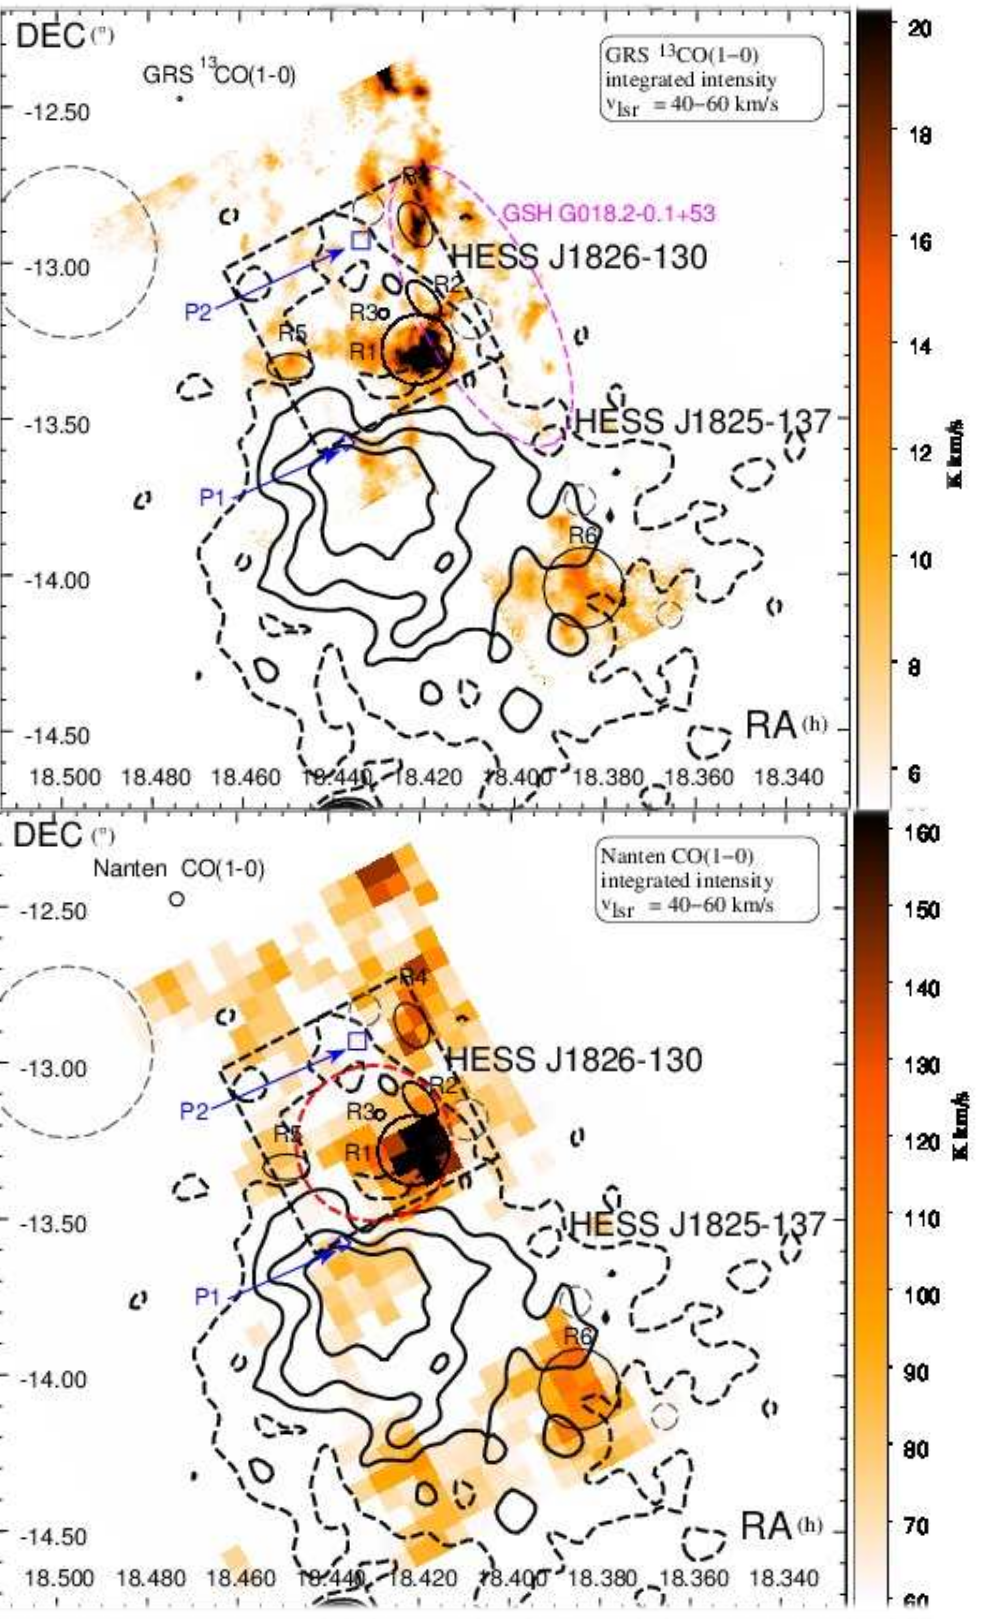
\includegraphics[width=0.45\textwidth]{06_Interstellar_Medium/Images/18252.png}
    \caption{$^{13}$CO$\qty(1-0)$ (\textit{top}) and $^{12}CO\qty(1-0)$ (\textit{bottom}) integrated intensity between velocity range $40-60~\si{\kilo\meter\per\second}$ (equivalent to $3.5-4.5~\kpc$) towards \mbox{HESS\,J1825-137}. HESS TeV gamma-ray emission contours are shown by the solid and dashed black contours. Image courtesy of \citep{2016MNRAS.458.2813V}}
	\label{fig:chapter_6_1825_gas}
\end{wrapfigure}

The interstellar medium (ISM) is the gas existing in between stars and other astrophysical objects in the Galaxy. The ISM includes atomic and molecular gas, dust, plasma and cosmic rays and accounts for $10-15\%$ of the total mass in the Galactic disc \citep{2001RvMP...73.1031F}. By number, the chemical composition of the ISM is $90.8\%$ hydrogen, $9.1\%$ helium and $0.12\%$ heavier elements \citep{2001RvMP...73.1031F}. By mass hydrogen makes up $70.4\%$ of the ISM with the remainder being $28.1\%$ Helium and $1.5\%$ heavier elements. As cosmic rays and gamma rays leave their place of birth, they must traverse the ISM before being observed at Earth.
\par~\par 
As discussed in \autoref{sec:01_1825_1826}, \mbox{HESS\,J1825-137} lies at a distance of $4.0~\kpc$  \citep{2006A&A...460..365A}. \autoref{fig:chapter_6_1825_gas} shows carbon monoxide (CO) gas lying in range $3.5-4.5~\kpc$ towards \mbox{HESS\,J1825-137} and \mbox{HESS\,J1826-130}, where CO is used as a trace for molecular hydrogen (see \autoref{sec:06_molecular_tracers}). The ISM gas towards this region will influence the transport of cosmic rays escaping the PWN (and SNR) associated with \mbox{HESS\,J1825-137} and the subsequent gamma-ray emission from this region. Therefore, the ISM must be considered in any study towards this region. This chapter will discuss properties of the ISM as well as the observatories whose data products were used in this thesis.
\newpage  %I need to put this or elese it looks nasty (due to the wrap figure)
\section{Detecting the interstellar medium}

The ISM gas towards \mbox{HESS\,J1825-137} influences the rate at which cosmic rays propagate and their cooling time (see \autoref{sec:chapter1_non_thermal_emission}). Radiation theory describes how particles (photons and cosmic rays) interact with a medium during propagation \citep{2011piim.book.....D}. As photons travel through the ISM before detection at Earth, it is important to characterise how the interstellar gas affects observations.

\subsection{Specific Intensity, Specific Flux and Bolometric flux}

Firstly, this section will define fundamental concepts.
\par~\par 
\noindent Let a telescope with detecting area $\dd{A}$ observe photons (in frequency range $\nu + \dd{\nu}$ and energy range $E+\dd{E}$) from a source within solid angle $\dd{\Omega}$ at orientation $\theta$ in time $\dd{t}$ (see \autoref{fig:telescope_basic_diagram2}).

\begin{SCfigure}[0.42][h!]
	\centering
	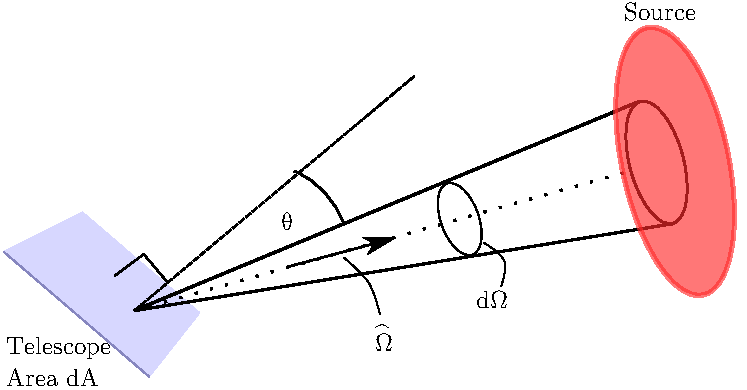
\includegraphics[width=0.7\textwidth]{06_Interstellar_Medium/Images/Theory/intensity.pdf}
	\caption{A basic illustration of a telescope with area $\dd{A}$ observing a cloud of ISM gas with solid angle $\dd{\Omega}$ at at orientation $\theta$.}
	\label{fig:telescope_basic_diagram2}
\end{SCfigure}
\noindent The amount of photons arriving within solid angle $\dd{\Omega}$ is described by the the specific intensity:

\begin{equation}
	\begin{aligned}
		I_\nu\qty(\hat{\Omega})&=\frac{\dd{E}}{\dd{A}\dd{t}\dd{\nu}\dd{\Omega}}\quad\qty[\si{\watt\per\meter\squared\per\hertz\per\steradian}]\text{ .}
	\end{aligned}
\end{equation}
% \noindent Alternative units for specific intensity are $\si{\erg\per\second\per\centi\meter\squared\per\hertz\per\steradian}$.
\par~\par 
\noindent The net specific flux, $F_\nu$, is obtained by integrating the specific intensity over the entire source:

\begin{equation}
	\begin{aligned}
		F_\nu &=\oint I_\nu\qty(\hat{\Omega})\cos\theta\dd{\Omega}\quad\qty[\si{\watt\per\meter\squared\per\hertz}]\text{ .}
	\end{aligned}
\end{equation}
\noindent A common unit for the specific flux in the radio domain is the Janksy ($\si{Jy}$) where $1~\si{Jy}=10^{-26}~\si{\watt\per\meter\squared\per\hertz} = 10^{-23}~\si{\erg\per\centi\meter\squared\per\second\per\hertz}$. If the specific intensity is isotropic ($I_\nu\qty(\hat{\Omega})=I_\nu$) then $\oint \cos\theta\dd{\Omega}=0$ and the specific flux is zero. If the telescope is pointed towards the source ($\cos\theta=1$) and the source is uniformly bright ($I_\nu\qty(\hat{\Omega})=I_\nu$), then the specific flux is simply:
\begin{equation}
	\begin{aligned}
		F_\nu&=I_\nu\Delta\Omega\text{ .}
	\end{aligned}\label{eq:specifc_flux_uniform_source}
\end{equation}
\noindent The bolometric flux, $F$, is the specific flux integrated over all frequencies:

\begin{equation}
	\begin{aligned}
		F&=\int F_\nu \dd{\nu}~\quad\qty[\si{\watt\per\meter\squared}]\text{ ,}
	\end{aligned}
\end{equation}
\noindent and is a measure of the total amount of photons emitted by a source.

\subsection{Radiative Transfer}

Let a cloud with thickness $\dd{s}=c\dd{t}$ (volume $\dd{V}=\dd{A}c\dd{t}$) and particle number density $n$ be illuminated by a background source with specific intensity $I_\nu$ on area $\dd{A}$ (see \autoref{fig:photon_energy_density}).

\begin{figure}[H]
	\centering
	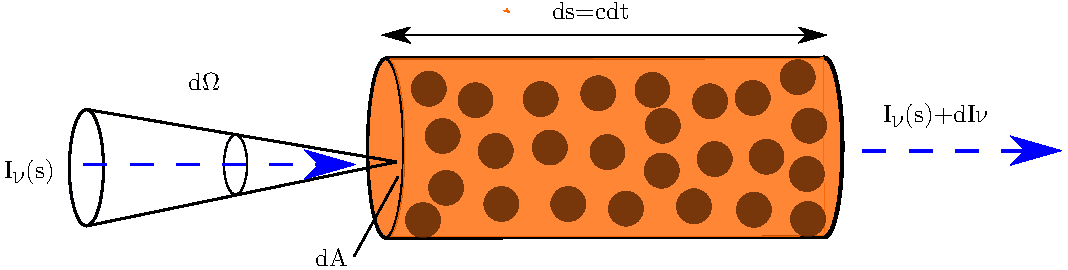
\includegraphics[width=\textwidth]{06_Interstellar_Medium/Images/Theory/radiative_transfer.pdf}
	\caption{A cloud of thickness $\dd{s}$ is illuminated by a background source with intensity $I_\nu\qty(s)$. Photons of frequency $\nu$ are emitted and re-emitted by particles (dark circles) within the cloud, changing the intensity by $\dd{I_\nu}$}
	\label{fig:photon_energy_density}
\end{figure}
\noindent The cloud contains $n\dd{V}$ particles with each particle having an absorption cross section $\sigma_\nu$ for radiation of frequency $\nu$. The total absorption area of the cloud can be described by $n\dd{s}\dd{A}\sigma_\nu$, giving the fraction of photons absorbed to be:

\begin{equation}
    \begin{aligned}
        f_\text{absorbed}&=n\dd{s}\dd{A}\sigma_\nu/\dd{A} \\
        &=n\dd{s}\sigma \text{ .}
    \end{aligned}
\end{equation}
\noindent Therefore, the change in intensity due to absorption is:

\begin{equation}
    \begin{aligned}
        \dd{I_{\nu,\text{absorbed}}}&=- \frac{n\dd{V}\sigma_\nu}{\dd{A}} \\
        &= - \alpha_\nu I_\nu \dd{s}\text{ ,}
    \end{aligned}
\end{equation}
\noindent where $\alpha_\nu=n\sigma_\nu~\qty[\si{\per\meter}]$ is the absorption coefficient. The absorption mean free path is the distance a photon will travel in the cloud before absorption and is given by:

\begin{equation}
	\begin{aligned}
		\ell_\nu &=\alpha_\nu^{-1}\text{ .}
	\end{aligned}
\end{equation}

\noindent If the cloud in \autoref{fig:photon_energy_density} has emission coefficient $j_\nu$
$\qty[\si{\watt\per\meter\cubed\per\hertz\per\steradian}]$ (i.e. the power emitted at frequency $\nu$ by an infinitesimal volume $\dd{V}$), the specific intensity emitted by the cloud is:

\begin{equation}
	\begin{aligned}
		\dd{I_{\nu\text{, emitted}}}&=j_\nu \dd{s} \\
		\therefore I_{\nu\text{, emitted}} &= \int j_\nu \dd{s} \text{ .}
	\end{aligned}\label{eq:emission_coefficient}
\end{equation}
\noindent Giving the total change in intensity in the cloud to be:

\begin{equation}
	\begin{aligned}
		\dv{I_\nu}{s}&=-\alpha_\nu\qty(s)I_\nu\qty(s)+j_\nu\qty(s) \\
		\frac{\dd{I_\nu}}{\alpha_\nu\dd{s}}&=-I_\nu\qty(s)+\frac{j_\nu\qty(s)}{\alpha_\nu\qty(s)} \\
		\dv{I_\nu}{\tau}&=-I_\nu\qty(\tau_\nu)+S\qty(\tau_\nu)\text{ ,}
	\end{aligned} \label{eq:radiative_transfer}
\end{equation}
\noindent where $\tau_\nu$ is the optical depth defined by:

\begin{equation}
	\begin{aligned}
		\dd{\tau_\nu}&=\alpha_\nu \dd{s}\text{ ,}
	\end{aligned}
\end{equation}
\noindent and $S_\nu\qty(\tau_\nu)=j_\nu\qty(s)/\alpha_\nu\qty(s)$ is the source function of the cloud. \autoref{eq:radiative_transfer} has solution:

\begin{equation}
	\begin{aligned}
		I_\nu\qty(\tau_\nu)&=\exp\qty(-\tau_\nu)\qty[I_\nu\qty(0)+\int_{0}^{\tau_\nu}\exp\qty(\tau'_\nu)S_\nu\qty(\tau'_\nu)\dd{\tau'_\nu}] \text{ .}
	\end{aligned} \label{eq:radiative_transfer_solution1}
\end{equation}

If there is no emission from the cloud, $S_\nu\qty(\tau_\nu)=j_\nu\qty(s)=0$, then the specific intensity can be described by:

\begin{equation}
    \begin{aligned}
        I_\nu\qty(\tau_\nu)&=I_\nu\qty(0)\exp\qty(-\tau_\nu)\text{ .}
    \end{aligned}
\end{equation}
\noindent i.e. the specific intensity of the background source after absorption by the cloud. If the emission/absorption of the cloud is uniform, $S_\nu\qty(\tau_\nu)=S_\nu$, \autoref{eq:radiative_transfer_solution1} becomes:

\begin{equation}
	\begin{aligned}
		I_\nu\qty(\tau_\nu)&=I_\nu\qty(0)\exp\qty(-\tau_\nu)+S_\nu\qty(1-\exp\qty(-\tau_\nu)) \\
        &=S_\nu + \exp\qty(-\tau_\nu)\qty[I_\nu\qty(0)-S_\nu] \text{ .}
	\end{aligned} \label{eq:radiative_transfer_solution2}
\end{equation}
\noindent If the cloud is optically thick, $\tau_\nu\gg 1$:

\begin{equation}
    \begin{aligned}
        I_\nu\qty(\tau_\nu)&\approx S_\nu\text{ .}
    \end{aligned}
\end{equation}
\noindent This is when a medium is opaque and only photons emitted by the cloud are observed. If optically thin, $\tau \ll 1$, then the exponential in \autoref{eq:radiative_transfer_solution2} can be approximated by $\exp(-\tau_\nu)\approx 1-\tau_\nu$ and the observed specific intensity becomes:

\begin{equation}
	\begin{aligned}
		I_\nu\qty(\tau_\nu)&=I_\nu\qty(0)\qty(1-\tau_\nu)+S_\nu\tau_\nu\text{ .}
	\end{aligned}
\end{equation}

\subsection{Black Bodies} \label{sec:06_blackbodies}

Thermal radiation is the emitted radiation due to the random motion/kinetic energy (i.e. temperature) of its particles. Thermal sources such as stars, CMB and interstellar dust can be described by an object emitting radiation with frequency $\nu$ at temperature $T$. A black body is an idealised object that absorbs all incoming radiation. A black body at temperature $T$ emits radiation at an intensity described by Planck's distribution:

\begin{equation}
	\begin{aligned}
		B_\nu\qty(T)&= \frac{2h\nu^3/c^2}{\exp(h\nu/kT)-1}\quad\qty[\si{\watt\per\steradian\per\meter\squared\per\hertz}] \text{ ,}
	\end{aligned}
\end{equation}
\noindent  where $h$ is Planck's constant and $k$ is Boltzmann's constant. The integrated intensity over all frequencies from a black body is given by the Stefan-Boltzman Law:

\begin{equation}
	\begin{aligned}
		F&=\sigma T^4~\qty[\si{\watt\per\meter\squared}]\text{ ,}
	\end{aligned}
\end{equation}
\noindent with $\sigma$ being the Stefan–Boltzmann constant. Objects in thermal equilibrium emit radiation in a manner that is dependent on their temperature. For an `ideal' black body to be in thermal equilibrium with its surroundings, the incoming intensity ($I\qty(0)=B_\nu$) and emitted intensity ($I\qty(\tau)=B_\nu$) are equal. \autoref{eq:radiative_transfer_solution2} becomes:

\begin{equation}
    \begin{aligned}
        B_\nu\qty(T)&=S_\nu\qty(T) + \exp\qty(-\tau_\nu)\qty[B\qty(T)-S_\nu\qty(T)] \text{ .}\\
    \end{aligned}
\end{equation}
\noindent This is only true for all $\tau$ when:

\begin{equation}
    \begin{aligned}
    	\therefore S_\nu\qty(T) &= B_\nu\qty(T)=\frac{j_\nu\qty(T)}{\alpha_\nu\qty(T)}\text{ .}
    \end{aligned} \label{eq:kirchoffs_law}
    \end{equation}
\noindent \autoref{eq:kirchoffs_law} is known as Kirchoff's law of radiation. Hence, the emission of a black body can be described by:

\begin{equation}
    \begin{aligned}
        I_\nu\qty(\tau_\nu)&=I_\nu\qty(0)\exp(-\tau_\nu)+B_\nu\qty(T)\qty[1-\exp(-\tau_\nu)]\text{ .}
    \end{aligned} \label{eq:chapter_6_black_body_emission}
\end{equation}
\noindent For an optically thick medium ($\tau\gg 1$) then:

\begin{equation}
    \begin{aligned}
        I_\nu\qty(\tau_\nu)\approx B_\nu\qty(T) \text{ ,}
    \end{aligned}
\end{equation}
\noindent and the medium can be approximated as a black body. Molecular tracers such as CO (see \autoref{sec:06_molecular_tracers}) emit radiation in the radio band. At these low frequencies ($h\nu\ll kT$ and $\exp(h\nu/kT)\approx1+h\nu/kT$) , the intensity of a black body can be approximated by:

\begin{equation}
    \begin{aligned}
        B_\nu\qty(T)&=\frac{2\nu^2kT}{c^2}\text{ .}
    \end{aligned}
\end{equation}

In radio astronomy, brightness temperature ($T_B$) is often used to measure intensity where $B_\nu(T_B)\equiv I_\nu$:

\begin{equation}
    \begin{aligned}
        T_B\qty(\nu)&=\frac{c^2}{2\nu^2 k}I_\nu\text{ .}
    \end{aligned} \label{eq:chapter_6_brightness_temp}
\end{equation}
\noindent Brightness temperature is the temperature that an ideal black body in thermal equilibrium would have in order to emit intensity $I_\nu$. For example, brightness temperature can be used to describe molecular clouds with temperatures $\approx 10~\si{K}$ for frequencies $\ll 208~\si{\giga\hertz}$ \citep{2011hea..book.....L}.

\subsection{Spectral Line Excitation and Emission} \label{sec:interstellar_medium_excitation_emission}

\begin{figure}[h]
	\centering
	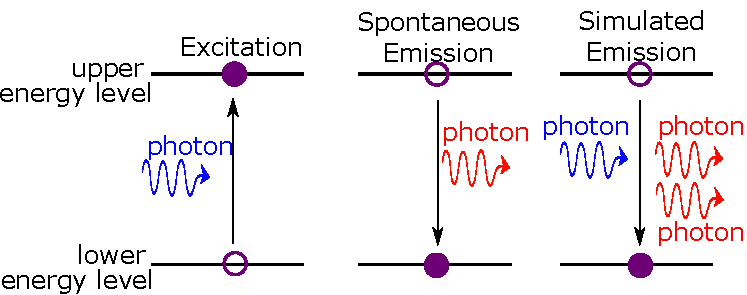
\includegraphics[width=0.7\textwidth]{06_Interstellar_Medium/Images/Theory/emission.pdf}
	\caption{(\textit{left}) Excitation of an electron from a low to higher energy level due to absorption of energy from a photon. (\textit{middle}) The emission of a photon when an electron spontaneously decays to a lower energy level. (\textit{right}) An incident photon interacts with an excited atom, causing the electron to decay to a lower energy level and emit a photon.}
	\label{fig:absorption_emission}
\end{figure}

Atoms populate their electrons in orbitals, from low to high energy levels. The stable state (or ground state) of an atom occurs when the electrons occupy their lowest energy level. The absorption of a photon can raise the energy level of an atom to a higher one (see left panel of \autoref{fig:absorption_emission}) and can only occur when the photon has energy equal to the energy difference between the two levels ($h\nu=E_2-E_1$, where $E_2>E_1$). An atom can exist in this excited state for a short period of time until it decays to a lower energy level and emits a photon with energy equal to the energy difference between the initial and final energy level (see middle panel if \autoref{fig:absorption_emission}). This is known as spontaneous emission. The Einstein coefficient, $A_{if}$, gives the probability per unit time for spontaneous emission from state $i$ to state $f$ and releasing photon of frequency $\nu_{if}$. If the number density of atoms in state $i$ is $n_i$, then the emission coefficient is given by:

\begin{equation}
	\begin{aligned}
		j_\nu&=\frac{n_ih\nu_{if}A_{if}}{4\pi}\Phi\qty(\nu)\text{ .}
	\end{aligned} \label{eq:interstellar_medium_emission_coefficient}
\end{equation}
\noindent For example, H$\alpha$ emission occurs when the electron in an excited hydrogen atom decays from the third to second energy level. As a result H$\alpha$ emission is used as a tracer for ionised gas. In its neutral state, a hydrogen atom consists of one electron-proton pair with their spins either parallel or antiparallel. The hydrogen atom may spontaneously switch the spin of its electron from parallel to antiparallel to the proton spin and release radiation with a wavelength of $21~\cm$ known as the HI line. This HI line can be used to probe neutral hydrogen gas in the Galaxy and beyond.
\par~\par
Stimulated emission occurs when an external photon interacts with an excited atom causing an emission of a photon with the same wavelength, polarisation and direction as the initial photon (see \autoref{fig:absorption_emission}). The initial photon must have -- for stimulated emission to occur.

\section{Probing the interstellar medium} 

\subsection{Molecular Tracers} \label{sec:06_molecular_tracers}

H$_2$ is the most abundant molecule in the Galaxy, consisting of two bound hydrogen atoms. Molecular hydrogen has 14 vibration energy levels that require high temperatures ($>5000~\si{\kelvin}$) for excitation \citep{2011piim.book.....D}. However, observed molecular clouds have temperatures $\approx 10-20~\si{\kelvin}$ \citep{2001RvMP...73.1031F} and the transition rate to higher energy levels are quite low. Moreover, the symmetry of H$_2$ molecules makes dipole radiation `forbidden' while electric quadruple radiation is possible with very low probability \citep{2011piim.book.....D}.
\par~\par 
The two nuclei in $H_2$ molecules rotate around their centre of mass with angular momentum components $J_x$, $J_y$ and $J_z$ \citep{alma99117570501811} and total rotational energy:

\begin{equation}
    \begin{aligned}
        E_\text{rot}&=\frac{J_x^2}{2I_x}+\frac{J_y^2}{2I_y}+\frac{J_z^2}{2I_z}\text{ ,}
    \end{aligned} \label{eq:chapter_6_molecular_rotation_energy}
\end{equation}
\noindent where $I_{i}$ is the moment of inertia in the ith axis ($i=x,y,z$). For linear rotors (e.g. H$_2$, CO)  $I_x\ll I_y=I_z$ where $I_x$ can be treated as zero \citep{alma9928060792901811}. \autoref{eq:chapter_6_molecular_rotation_energy} becomes:

\begin{equation}
    \begin{aligned}
        E_\text{rot}&=\frac{J^2}{2I}\text{ ,}
    \end{aligned}
\end{equation}
\noindent where the eigenvalue of $J^2$ is $j\qty(j+1)\hbar^2$ \citep{alma99117570501811}. Hence:

\begin{equation}
    \begin{aligned}
        E_\text{rot}&=\frac{\hbar^2}{2I}j\qty(j+1)\text{ ,}
    \end{aligned}
\end{equation}
\noindent with $\hbar=h/\qty(2\pi)$ and $j=0$, $1$, $2$... For a $H_2$ molecule absorbing/emitting a photon (with energy $E_\gamma$) that causes a change in energy level, the difference in energy levels is given by:

\begin{equation}
    \begin{aligned}
        E_\gamma=\Delta E_{rot} = \frac{j\hbar^2}{I}\text{ .}
    \end{aligned}
\end{equation}
\noindent For molecular hydrogen, temperatures greater than $100~\si{\kelvin}$ are required for rotational energy excitation. Hence, molecules within the majority of quiescent $H_2$ clouds exist in their vibrational and rotational ground state. 
\par~\par 
After H$_2$, the second most abundant molecule is CO, following a  CO/H$_2$ abundance ratio of $10^{-4}$ in molecular clouds \citep{1994ApJ...428L..69L}. The transition between the ground and first rotational energy level ($J=1-0$) for CO requires much lower temperatures $\approx 5~\si{\kelvin}$, corresponding to photons being emitted at frequency $115~\si{\giga\hertz}$ ($\lambda=2.6~\si{\milli\meter}$) \citep{alma9927598238601811}. Therefore, carbon monoxide can be used as a tracer for molecular hydrogen (see \citep{Bolatto2013}).
\par~\par
High-frequency radio telescopes, such as Nanten (see \autoref{sec:NANTEN}), observe the intensity of molecular CO in units of brightness temperature (see \autoref{eq:chapter_6_brightness_temp}). To interpret the amount of gas towards a particular region, the CO$(1-0)$ brightness intensity is converted to a column density ($\si{\per\centi\meter\squared}$) of molecular hydrogen through the conversion factor $X_\text{CO}$:

\begin{equation}
	\begin{aligned}
		N_{H_2}&=X_\text{CO}W_\text{CO}\text{ ,}
	\end{aligned}
\end{equation}
\noindent where $W_\text{CO}$ is the integrated intensity in units $\si{\kilo\meter\per\second}$. The conversion factor is often assumed to be constant ($X_\text{CO}=1.5\times 10^{20}~\si{\per\centi\meter\squared\per\kelvin\per\kilo\meter\squared\second}$) across the Galactic plane, but it is known to vary with galactocentric radius \citep{2004A&A...422L..47S}. The number density, $n_H$, and mass, $M_H$, of hydrogen in a cloud with column density $N_{H_2}$ are respectively:

\begin{equation}
	\begin{aligned}
		n_H&=\frac{\mu N_{H_2}}{\Delta z} \label{eq:06_density_gas} \\
		M_H&=n_Hm_pV\text{ ,}
	\end{aligned}
\end{equation}
\noindent $\Delta z$ is the width of the cloud along the line of sight, $V$ is the volume of the cloud and $m_p$ is the mass of the proton. The weight factor, $\mu$, of a gas cloud is:

\begin{equation}
    \begin{aligned}
        \mu&=\sum_Z n A_r\text{ ,}
    \end{aligned}
\end{equation}
\noindent where $\sum_Z$ sums over the molecules present in the cloud, $n$ is the number of atoms present in the molecule ($n=2$ for molecular hydrogen) and $A_r$ is the atomic weight ($A_r\approx1$ for hydrogen and $A_r\approx 4$ for helium). For a gas cloud with $20\%$ Helium component, the weight factor is $2.8$.

\subsection{Doppler Shift}

\autoref{sec:06_molecular_tracers} discussed how atomic and molecular gas emit photons with wavelengths dependent on their atomic structure. However, the bulk movement of gas clouds around the Galactic Center (GC) will shift the frequency of photons due to the Doppler effect. The shift in frequency is described by:

\begin{equation}
    \begin{aligned}
        \nu = \frac{c+V_\text{obs}}{c+V}\nu_0\text{ ,}
    \end{aligned}
\end{equation}
\noindent where $\nu$ is the observed frequency, $\nu_0$ is the emitted frequency, $V$ is the veloicty of the gas cloud and $V_\text{obs}$ is the velocity of the observer. Therefore, a shift in frequency can be represented as a velocity in respect to a rest frame:

\begin{equation}
    \begin{aligned}
        V_\text{LSR}=c\frac{\qty(\nu_0-\nu)}{\nu_0}\text{ .}
    \end{aligned}
\end{equation}
\noindent The typical rest frame used is the local standard of rest (LSR), taken at the point coincident with the Sun orbiting around the GC in a perfect circular orbit.

\subsection{Galactic Rotation Curve} \label{sec:06_galactic_rotation}

Matter rotates around the GC with an average tangential speed of $\Theta_0\approx 220~\kmpersec$. The Galactic rotation curve is an empirical model (see \autoref{fig:Galactic_rotation_model}) that relates the galactocentric radius (distance to the GC) of an object to its observational velocity.
\begin{figure}[h!]
	\centering
	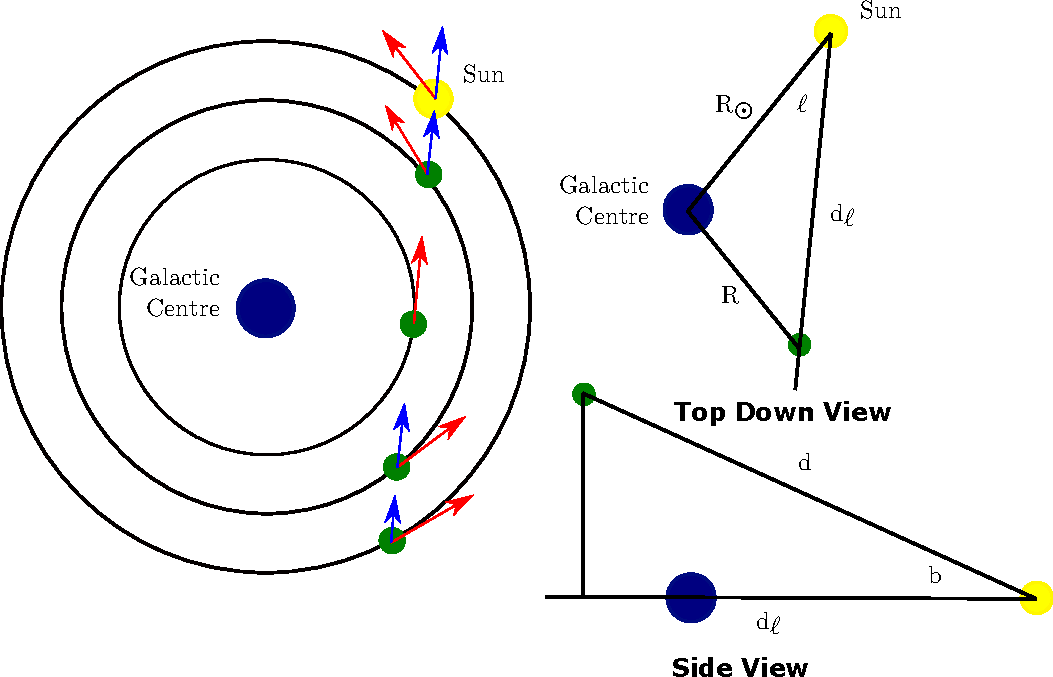
\includegraphics[width=1.0\textwidth]{06_Interstellar_Medium/Images/Theory/galaxy_combined.pdf}
	\caption{(\textit{Left}) Rotation of the Galaxy around the GC (dark blue circle) with the yellow circle as the Sun, the red arrows are the tangential velocity of the green objects (e.g. gas cloud) and the blue arrows are their velocities projected along the line of sight to the Sun. (\textit{Right}) Geometry of an object at Galactic longitude $\ell$, Galactic latitude $b$ and distance $d$ from the Sun.}
	\label{fig:Galactic_rotation_model}
\end{figure}
Using HI clouds, \cite{1993A&A...275...67B} found that the measured velocity of a cloud, $V_\text{LSR}$, can be transformed into circular rotation velocity, $\Theta_0$, via:
\begin{equation}
\begin{aligned}
    V_\text{LSR}&=\qty(\frac{\Theta R_\odot}{R}-\Theta_\odot)\sin\ell \cos b\text{ ,}
\end{aligned} \label{eq:chapter_6_brand_blitz_velocity}
\end{equation}
\noindent where $\ell$ and $b$ are the Galactic coordinates of the cloud, $R$ and $\Theta$ are the galactocentric distance and circular rotation velocity of the cloud respectively and $R_\odot$ is the galactocentric distance of the Sun. The circular rotation velocity is related to the galactocentric distance by:

\begin{equation}
    \begin{aligned}
        \frac{\Theta}{\Theta_\odot}&=a_1 \qty(\frac{R}{R_\odot})^{a_2}+a_3\text{ ,}
    \end{aligned} \label{eq:06_circular_rotatoin_velocity}
\end{equation}
\noindent where $a_1=1.00767$, $a_2=0.0394$ and $a_3=0.00712$ are the values found by \cite{1993A&A...275...67B}. For a cloud with circular rotation velocity $V_\text{LSR}$ at coordinate $\ell$ and $b$, \autoref{eq:chapter_6_brand_blitz_velocity} and \autoref{eq:06_circular_rotatoin_velocity} can be solved numerically to find $R$ and $\Theta$. Using simple trigonometry (see \autoref{fig:Galactic_rotation_model}), the distance to the GC for an object at distance $d$ and coordinates $\qty(\ell,b)$ is given by:

\begin{equation}
    \begin{aligned}
        R^2&=d^2\cos^2b+R_\odot^2-2dR_\odot\cos b\cos\ell\text{ ,}
    \end{aligned}
\end{equation}
\noindent which gives a near and far distance to the cloud (see \autoref{fig:Galactic_rotation_model}). In general, the near distance is taken to be the solution; a source further away is more likely to have its emission being obstructed by closer gas. Moreover, a distant source will appear dimmer than a nearby source due to intensity following the inverse square law ($I\propto d^{-2}$).
\par~\par 
Other parameterisations of the Galactic rotation curves include \cite{1985ApJ...295..422C}, who analysed the Massachusetts-Stony Brook Galactic plane CO survey \citep{1985ApJ...289..373S}. \cite{1996MNRAS.281...27P} provided a `universal rotation curve' which includes contributions from a stellar disk and a dark halo. Alternatively \cite{2014ApJ...783..130R} describes the Galactic rotation curve as a polynomial:

\begin{equation}
    \begin{aligned}
        \Theta\qty(R)&=a_{p1}+a_{p2}\rho+a_{p3}\rho^3 \\
        \rho &=\frac{R}{R_0}-1\text{ ,}
    \end{aligned}
\end{equation}
\noindent with $a_{p1}=[241\pm 9]~\kmpersec$, $a_{p2}=0.5\pm 3.7$ and $a_{p3}=-15.1\pm 8.4$. 
\par~\par 
The velocity in \autoref{eq:chapter_6_brand_blitz_velocity} describes the circular rotation velocity of an object around the Galaxy. However, the velocity measured at Earth is the combined velocity due to Galactic rotation and local individual gas motion (e.g. due to stellar winds, SNR shock fronts). \cite{1993A&A...275...67B} noted that residuals of modelled gas with respect to the Galactic rotation curve can be as large as $40~\kmpersec$ with the average being around $12.8~\kmpersec$. This is significant compared to the Nanten observatory (see \autoref{sec:NANTEN}), velocity resolution of $1~\kmpersec$, whose data products were used in this thesis. The uncertainty in the individual velocity of the gas will lead to large uncertainties in distances (hundreds of parsecs) to gas clouds.
\par~\par 
\begin{figure}
    \centering
    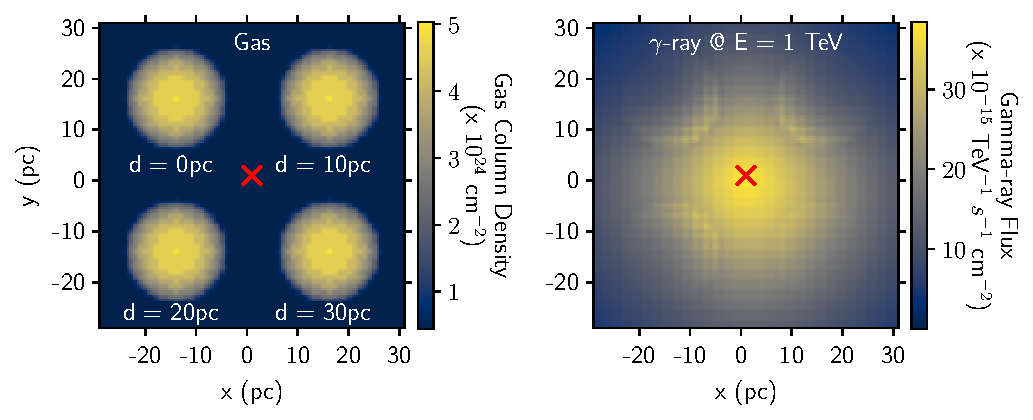
\includegraphics[width=1.0\textwidth]{06_Interstellar_Medium/Images/Theory/gas_distance_example.pdf}
    \caption{(\textit{Left}) Four spherical gas clouds located $4~\kpc$ from the Earth at distances $d$ along the line of sight (z-axis runs in/out of page) from a source of electrons (red cross). (\textit{Right}) Subsequent gamma-ray flux $40~\kiloyear$ after electron injection commences.}
    \label{fig:06_gas_distance_Example}
\end{figure}
The large uncertainties in distances to gas clouds (see \autoref{sec:06_galactic_rotation}) leads to a caveat in modelling the gas and magnetic field distribution (see \autoref{eq:sec_Bfield_gas}) around a cosmic-ray source. For example, consider a crude estimation in which the cosmic-ray intensity is described by an inverse square law $I\propto d^{-2}$ where $d$ is the distance from the accelerator. The cosmic-ray flux decreases with distance from a source, decreasing the subsequent gamma-ray energy flux from non-thermal emission (see \autoref{sec:chapter1_non_thermal_emission}). This can be seen in \autoref{fig:06_gas_distance_Example}, where four spherical gas clouds of number density $600~\centimeterminusthree$ ($B\approx 25~\si{\micro G}$) are located at different distances along the line of sight (z-axis) from a continuous source of electrons. The gamma-ray flux through IC interactions at $40~\kiloyear$ (suggested age of PWN \mbox{HESS\,J1925-137}, \cite{2011ApJ...742...62V}) decreases with increasing distance from the accelerator. Therefore, large uncertainties in distances to gas clouds will influence the modelled multiwavelength emission towards an accelerator.

\subsection{Magnetic fields in molecular clouds} \label{eq:sec_Bfield_gas}

The Zeeman effect (the splitting of spectral lines in the presence of a static magnetic field) can be used to measure the magnetic field strength in a medium. \cite{2010ApJ...725..466C} studied a population of quiescent clouds and related the magnetic strength of a cloud to its number density, $n$, through:

\begin{equation}
    \begin{aligned}
        B_\text{gas}\qty(n)=
    \begin{cases}
        B_0 \qquad &\text{, } n < n_0 \\
        B_0\qty(\frac{n}{n_0})^\alpha \qquad &\text{, } n > n_0
    \end{cases}\text{ ,}
    \end{aligned} \label{eq:ISM_crutchers}
\end{equation}
\noindent where clouds with a density above $n_0=300~\centimeterminusthree$ have an enhanced magnetic field described by a power-law regime with $B_0=10~\si{\micro G}$ and $\alpha=0.65$.
\par~\par 
Cosmic rays propagating through the ISM scatter off magnetic field turbulence and the overall motion is described by a random walk/diffusion (see \autoref{chapter_1_cr_propagation}), where the rate of diffusion is related to the strength of the magnetic field. From \autoref{eq:diffusion} and \autoref{eq:ISM_crutchers}, the rate that cosmic rays propagate through molecular clouds is anti-correlated with its density. i.e. cosmic rays travel through dense molecular clouds at a lower rate than less-dense clouds. Similarly, magnetic field turbulence in molecular clouds influences the rate of synchrotron energy loss (see \autoref{eq:01_leptonic_sync_energy_loss}). Cosmic ray electrons in dense molecular clouds will experience a higher rate of synchrotron (and Bremsstrahlung, see \autoref{eq:01_leptonic_brem_energy_loss}) interactions than less-dense clouds due to the enhanced magnetic field. Consequently, this decreases the `available' energy for IC interactions (see \autoref{eq:chapter_1_non_thermal_IC_e_energy_lost}). 

\subsection{H$\alpha$ emission}

\begin{SCfigure}[1][h!]
	\centering
	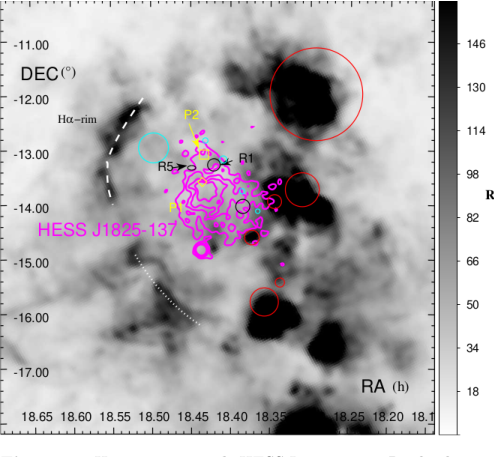
\includegraphics[width=0.5\textwidth]{06_Interstellar_Medium/Images/Theory/Fabien_Halpha.pdf}
	\caption{H$\alpha$ intensity towards \mbox{HESS\,J1825-137}. The dashed and dotted lines represent two H$\alpha$ rim-like features associated with the progenitor SNR of \mbox{HESS\,J1825-137}. Image courtesy of \citep{2016MNRAS.458.2813V}}
	\label{fig:06_1825_SNR}
\end{SCfigure}

Atomic hydrogen in clouds can be ionised by UV light from background stars to form HII regions, while shocks (SNRs), X-rays and cosmic rays leads to the ionisation of molecular hydrogen \citep{2011piim.book.....D}. Recombination of HII atoms and electrons may result in the the emission of light in the H$\alpha$ band (corresponding to a decay from the third to the second energy level). Hence, H$\alpha$ emission can be used as a tracer for ionised hydrogen gas (HII gas). Shocks associated with SNRs ionise hydrogen gas, leading to H$\alpha$ rim-like features similar to those towards \mbox{HESS\,J1825-137} (see \autoref{fig:06_1825_SNR}). Both structures are located $\approx 120~\pc$ from \mbox{PSR\,J1826-1334} which is consistent with the predicted SNR radius ($\approx 130~\pc$) as suggested by \cite{deJager2009}.
\par~\par
Ionised gas towards \mbox{HESS\,J1825-137} acts as a target for cosmic rays escaping from the PWN/SNR to undergo hadronic/leptonic interactions and emit gamma radiation. The following describes two different methods to trace the ionised hydrogen within molecular clouds.

\subsubsection{Method A}

For a spherical shell of gas located at distance $d$ from the Earth with thickness $\dd{\ell}$, the volume of the shell is given by:
\begin{equation}
    \begin{aligned}
        \dd{V}&=2\pi d^2 \dd{\ell}\text{ ,}
    \end{aligned}
\end{equation}
\noindent where photons emitted by the gas travel at the speed of light, hence $\dd{\ell}=c\dd{t}$. The total number of photons emitted in the shell in time $\dd{t}$ is related to the luminosity, $L$, via:

\begin{equation}
    \begin{aligned}
        \dd{N}&=L\dd{t}\text{ ,}
    \end{aligned}
\end{equation}
\noindent where the luminosity of the region of interest with solid angle $\omega$ is:
\begin{equation}
    \begin{aligned}
        L&=\frac{d^2}{10^{-10}}\Omega I\quad \qty[\text{photon/s}]\text{ ,}
    \end{aligned}
\end{equation}
\noindent with $I$ being the measured H$\alpha$ in Rayleigh units ($=10^{10}~\si{ph\per\meter\squared\per\second\per{column}}$). Assuming atoms are not re-excited by an external source, the density of photons emitted by ionised gas $u_\text{ph}$ is approximately equal to the ionised gas density, $n_\text{ion}$:

\begin{equation}
    \begin{aligned}
        n_\text{ion}\approx u_\text{ph}=\dv{N}{V}=\frac{L}{4\pi d^2 c}\text{ .}
    \end{aligned}
\end{equation}

\subsubsection*{Method B}

For photons of frequency $\nu$, the photon intensity ($I_\nu$) is related to the luminosity ($L$) through:

\begin{equation}
    \begin{aligned}
        I_\nu=L\frac{E_\nu}{\nu}=hL\text{ ,}
    \end{aligned}
\end{equation}
\noindent where $h$ is Planck's constant. For a cloud with thickness $s$, the emission coefficient is given by:

\begin{equation}
    \begin{aligned}
        j_\nu&=\frac{I_\nu}{s}\text{ ,}
    \end{aligned}
\end{equation}
\noindent assuming that the emission coefficient is constant throughout the gas. Hence, the density of atoms in the ith state emitting photons at frequency $\nu$ via spontaneous emission:

\begin{equation}
	\begin{aligned}
		n_i&=\frac{j_\nu \Omega_\text{Earth}}{E_\nu A\phi (\nu)}\text{ ,}
	\end{aligned}\label{eq:interstellar_medium_halpha_dens_2}
\end{equation}
where A is the Einstein coefficient, $\Omega_\text{earth}$ is the solid angle of Earth projected at source lying at distance $d$ and $\phi(\nu)$ is the spectral line shape normalised by:
\begin{equation}
	\begin{aligned}
		\int \phi(\nu)=1\text{ .}
	\end{aligned}
\end{equation}
Assuming that hydrogen atoms in the $n=3$ state emit mainly H$\alpha$ light; $\phi=0$ in all frequencies except when $\nu=\nu_{H\alpha}$. 

\subsection{Nanten2 Observatory} \label{sec:NANTEN}

\begin{figure} [h]
    \centering
    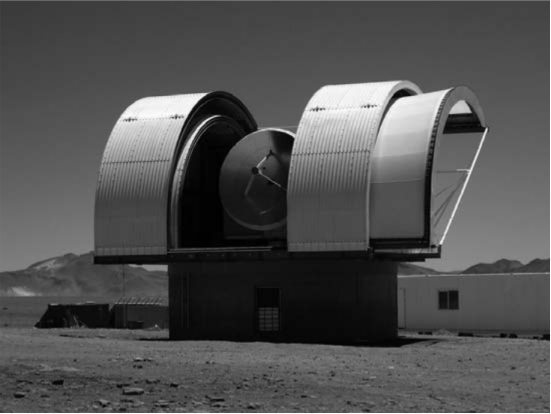
\includegraphics[width=0.7\textwidth]{06_Interstellar_Medium/Images/Observatories/Nanten2.pdf}
    \caption{Nanten2 telescope. Image courtesy of \cite{2006IAUSS...1E..21F}.}
    \label{fig:interstellar_medium_NANTEN}
\end{figure}

Nanten2 (Japanese for `Southern Sky') is an upgrade to the $4\m$ Nanten telescope originally located in Las Campanas before its relocation to the Atacama desert in Chile in 2004 \citep{2006IAUSS...1E..21F}. Nanten2 is located at altitude $4800~\m$ and consists of 33 adjustable aluminum panels on a light-weight carbon fiber back structure. Nanten2 is sensitive to atomic and molecular spectral lines  $100-880~\si{\hertz}$ and has angular resolution up to $2'6$ beam size \citep{2001PASJ...53L..45M}, allowing detailed observations of gas structures. Nanten2 has conducted multiple CO surveys of regions such as the Large Magellanic Cloud \citep{Kawamura_2009} and the Galactic plane \citep{2004ASPC..317...59M} covering velocity range $-300~\kmpersec$ to $300~\kmpersec$ with a velocity resolution up to $1.0~\kmpersec$.
\par~\par
\cite{2016MNRAS.458.2813V} conducted an ISM gas study towards PWN \mbox{HESS\,J1825-137} and \mbox{HESS\,J1826-130} utilising Nanten2 data. They found that the majority of gas towards this region is located in the velocity range $45-60~\kmpersec$ ($3.8-4.5~\kpc$) which is equivalent to the dispersion measure distance of the associated pulsar \mbox{PSR\,J1826-134}. \cite{2016MNRAS.458.2813V} noted six clouds of interest, named R1-R6, whose parameters are summarised in \autoref{tab:06_fabien_cloud_summary}. Cloud R1 was noted to show enhanced turbulence possibly due to the associated SNR shock or the formation of high-mass stars.
\begin{table}[h!]
    \caption{Derived parameters for clouds R1-R6 towards \mbox{HESS\,J1825-137} and \mbox{HESS\,J1826-130} utilising Nanten2 CO(J=1-0) from \cite{2016MNRAS.458.2813V}}
    \begin{threeparttable}
    \centering
    \begin{tabular}{cccccc}
        \toprule
        Cloud & RA ($\si{h}$) & DEC ($\si{\degree}$)& Radii ($''$) & $n_H$ ($\centimeterminusthree$) & $M_H$ ($M_\odot$) \\
        \midrule
        R1 & $18.421$ & $-13.282$ & $405\times 405$ & $960$ & $1.2\times 10^5$ \\
        R2 & $18.420$ & $-13.125$ & $135\times 270$ & $1200$ & $1.3\times 10^4$ \\
        R3 & $18.429$ & $-13.178$ & $64\times 64$ & $1600$ & $3.3\times 10^3$ \\
        R4 & $18.422$ & $-12.832$ & $175\times 280$ & $930$ & $1.6\times 10^4$ \\
        R5 & $18.449$ & $-13.336$ & $150\times 270$ & $680$ & $9.5\times 10^3$  \\
        R6 & $18.385$ & $-14.049$ & $460\times 460$ & $430$  & $7.6\times 10^4$ \\
        \bottomrule
    \end{tabular}
 %    \begin{tablenotes}
	% \item \textbf{References}
	% \item a: \citep{2020A&A...644A.112H}
 %    \end{tablenotes}
    \end{threeparttable}
    \label{tab:06_fabien_cloud_summary}
\end{table}